\section{MTProto}

\subsection{Telegram}
Telegram è un applicativo di messaggistica istantanea rilasciato nel 2013 da Pavel Durov e Nikolai Durov.
Proponendosi come alternativa al popolarissimo WhatsApp, Telegram è riuscito a ritagliarsi una buona fetta di mercato,
raggiungendo proprio recentemente i 700 milioni di utenti (Giugno 2022). \\
I servizi offerti sono molti e comprendono le semplici chat, i gruppi di più utenti e i canali usati per il broadcast.
Telegram fornisce inoltre un'API di facile utilizzo per lo sviluppo di bot e script automatici in grado di interagire
con il sistema. \\

Un altro aspetto particolarmente apprezzato, specialmente in alcuni ambiti, è la presunta sicurezza, privacy
e resistenza alla censura che questo social garantirebbe. \\
Alla base di tutto vi è un protocollo sviluppato da Telegram stesso, chiamato MTProto.

\subsection{Il protocollo MTProto}
\gls{mtproto} è un protocollo sviluppato da Telegram per la comunicazione sicura tra client e server. \\
La scelta di sviluppare un protocollo personalizzato invece che affidarsi a quelli già esistenti non è stata esente da critiche.
\gls{mtproto} è nato per affrontare alcune problematiche specifiche dell'ambito in cui opera:
\begin{itemize}
    \item garantire una certa affidabilità anche con le connessioni non all'altezza dei dispositivi mobili
    \item massimizzare la velocità nella gestione di grandi file, come foto e video
\end{itemize}

La prima versione di \gls{mtproto} presentava delle vulnerabilità che sono state evidenziate dal lavoro congiunto di due ricercatori dell'università di Aarhus \cite{inp:mtproto-v1-attacks}.
Sebbene nella pratica non si fosse riuscito ad individuare un attacco in grado di minare la sicurezza dei messaggi,
le criticità riscontrate nel protocollo sono state risolte con il rilascio della sua versione 2.0 nei client ufficiali v4.6 nel Dicembre del 2017 \cite{man:mtproto}. \\

Questa nuova versione ha superato diverse analisi volte a individuarne i punti deboli.
I risultati ne hanno comprovato la robustezza sia dal punto di vista crittografico \cite{inp:mtproto-attacks}
che dal punto di vista requisiti di sicurezza garantiti dal protocollo \cite{inp:mtproto-proverif}. \\

Va sottolineato inoltre che tutte le specifiche del protocollo sono pubbliche.
Ciò permette a chiunque di realizzare una propria versione del client in grado di interfacciarsi con tutti gli altri. \\

\subsection{Messaggi in MTProto}

\gls{mtproto} è un protocollo piuttosto complesso, ed è composto da molteplici sotto-protocolli, ciascuno con un compito specifico.
Si va dall'autenticazione e lo scambio di chiavi fra client e server, alla creazione di chiavi di sessione fra due client
al fine di realizzare una cifratura end-to-end, giusto per citare alcune funzioni previste. \\
Volendola vedere più ad alto livello, client e server si scambiano dei messaggi all'interno di una sessione.
La sessione è strettamente legata ad un dispositivo (o più precisamente, l'applicativo del dispositivo)
e all'identificativo dell'utente, utilizzato per l'autenticazione. \\
Una sessione può essere composta da più connessioni.
Non c'è alcuna garanzia che la risposta ad una richiesta venga fornita durante la stessa connessione o addirittura provenga dallo stesso \gls{ip},
sebbene sia il caso più comune, soprattutto nel caso di chiamate \gls{rpc}. \\

Vi sono diversi tipi di messaggi:
\begin{itemize}
    \item chiamate \gls{rpc} client-server
    \item risposte \gls{rpc} server-client
    \item messaggi di conferma di avvenuta ricezione
    \item messaggi di stato
    \item messaggi multi-parte composti da più messaggi, come ad esempio più chiamate \gls{rpc}
\end{itemize}

Scendendo ad un livello di inferiore, un messaggio è uno stream binario di dati con parole di 4 o 16 bytes (\autoref{fig:mtproto-message-1}).
I campi in testa sono riservati per i sistemi crittografici e di autenticazione. \\
Ogni messaggio contiene un identificatore univoco (64 bit), un sequence number (32 bit), la lunghezza (32 bit) del corpo in bytes e il corpo del messaggio (4 $\times$ n bytes).
I messaggi vengono poi cifrati e viene aggiunta un'intestazione che contiene un identificativo per la chiave (64 bit) e un identificativo del messaggio (128 bit). \\

\begin{figure}[!h]
    \includegraphics[width=\textwidth]{mtproto-msg-1.jpeg}
    \caption{Struttura di un messaggio in \gls{mtproto} \cite{man:mtproto}} \label{fig:mtproto-message-1}
\end{figure}

\subsection{Creazione della chiave di autorizzazione}
Il primo step previsto dal protocollo è la generazione della chiave di autorizzazione.
Con questa il client è in grado di autenticarsi agli occhi del sever. \\
La procedura si conclude con un \gls{dhe}, ed è così articolata (\autoref{fig:mtproto-sequence-auth}):
\begin{enumerate}
    \item il client invia una nonce al server
    \item il server risponde con la stessa nonce, una sua nonce, un valore $pq$ calcolato come prodotto fra due numeri primi,
          ed una lista di fingerprints RSA delle chiavi pubbliche del server
    \item il client decompone $pq$ nei suoi fattori primi $p, q$
    \item il client invia al server le due nonce che identificano la sessione, i valori $p, q$ e la lista di fingerprints.
          A ciò si aggiunge una fingerprint scelta fra quelle fornite dal server, con la quale cifrare tramite RSA un payload contenente
          la serializzazione binaria dei valori $pq, p, q$, nonce, nonce del server, ed una nuova nonce generata con una randomness crittografica
    \item il server risponde con le due nonce iniziali e un payload cifrato con AES256 con chiave $t_{temp}$ realizzata a partire dalla nuova nonce segreta inviata dal client tramite \gls{kdf}.
          Il payload contiene l'hash SHA1 della nuova nonce inviata dal client,
          un numero primo $2^{2047} < N < 2^{2048} : N, \frac{p-1}{2} \in \mathbb{N}$, un generatore $g$ di un gruppo ciclico con ordine $\frac{p-1}{2}$ e il valore $g^a$,
          dove $a$ è un numero casuale generato dal server
    \item il client genera in maniera sicura un numero random $b$ di 2048 bit ed invia al server le due nonce e un crittotesto
          cifrato con la chiave temporanea ${k_temp}$ contenente il valore $g^b$
    \item da questo momento in poi la chiave di autenticazione è uguale a $g^{ab}$, che sia il server che il client sono in grado di calcolare autonomamente
    \item l'hash della chiave di autenticazione è generato a partire dai 64 bit meno significativi dell'hash SHA1 della chiave di autenticazione
    \item se tutto è andato a buon fine, il server risponderà con un messaggio di conferma. Altrimenti, con un messaggio di errore o con un invito a riprovare
\end{enumerate}


\begin{figure}
    % generated by Plantuml 1.2022.0
    \definecolor{plantucolor0000}{RGB}{255,255,255}
    \definecolor{plantucolor0001}{RGB}{56,56,56}
    \definecolor{plantucolor0002}{RGB}{248,248,248}
    \definecolor{plantucolor0003}{RGB}{0,0,0}
    \definecolor{plantucolor0004}{RGB}{235,235,235}
    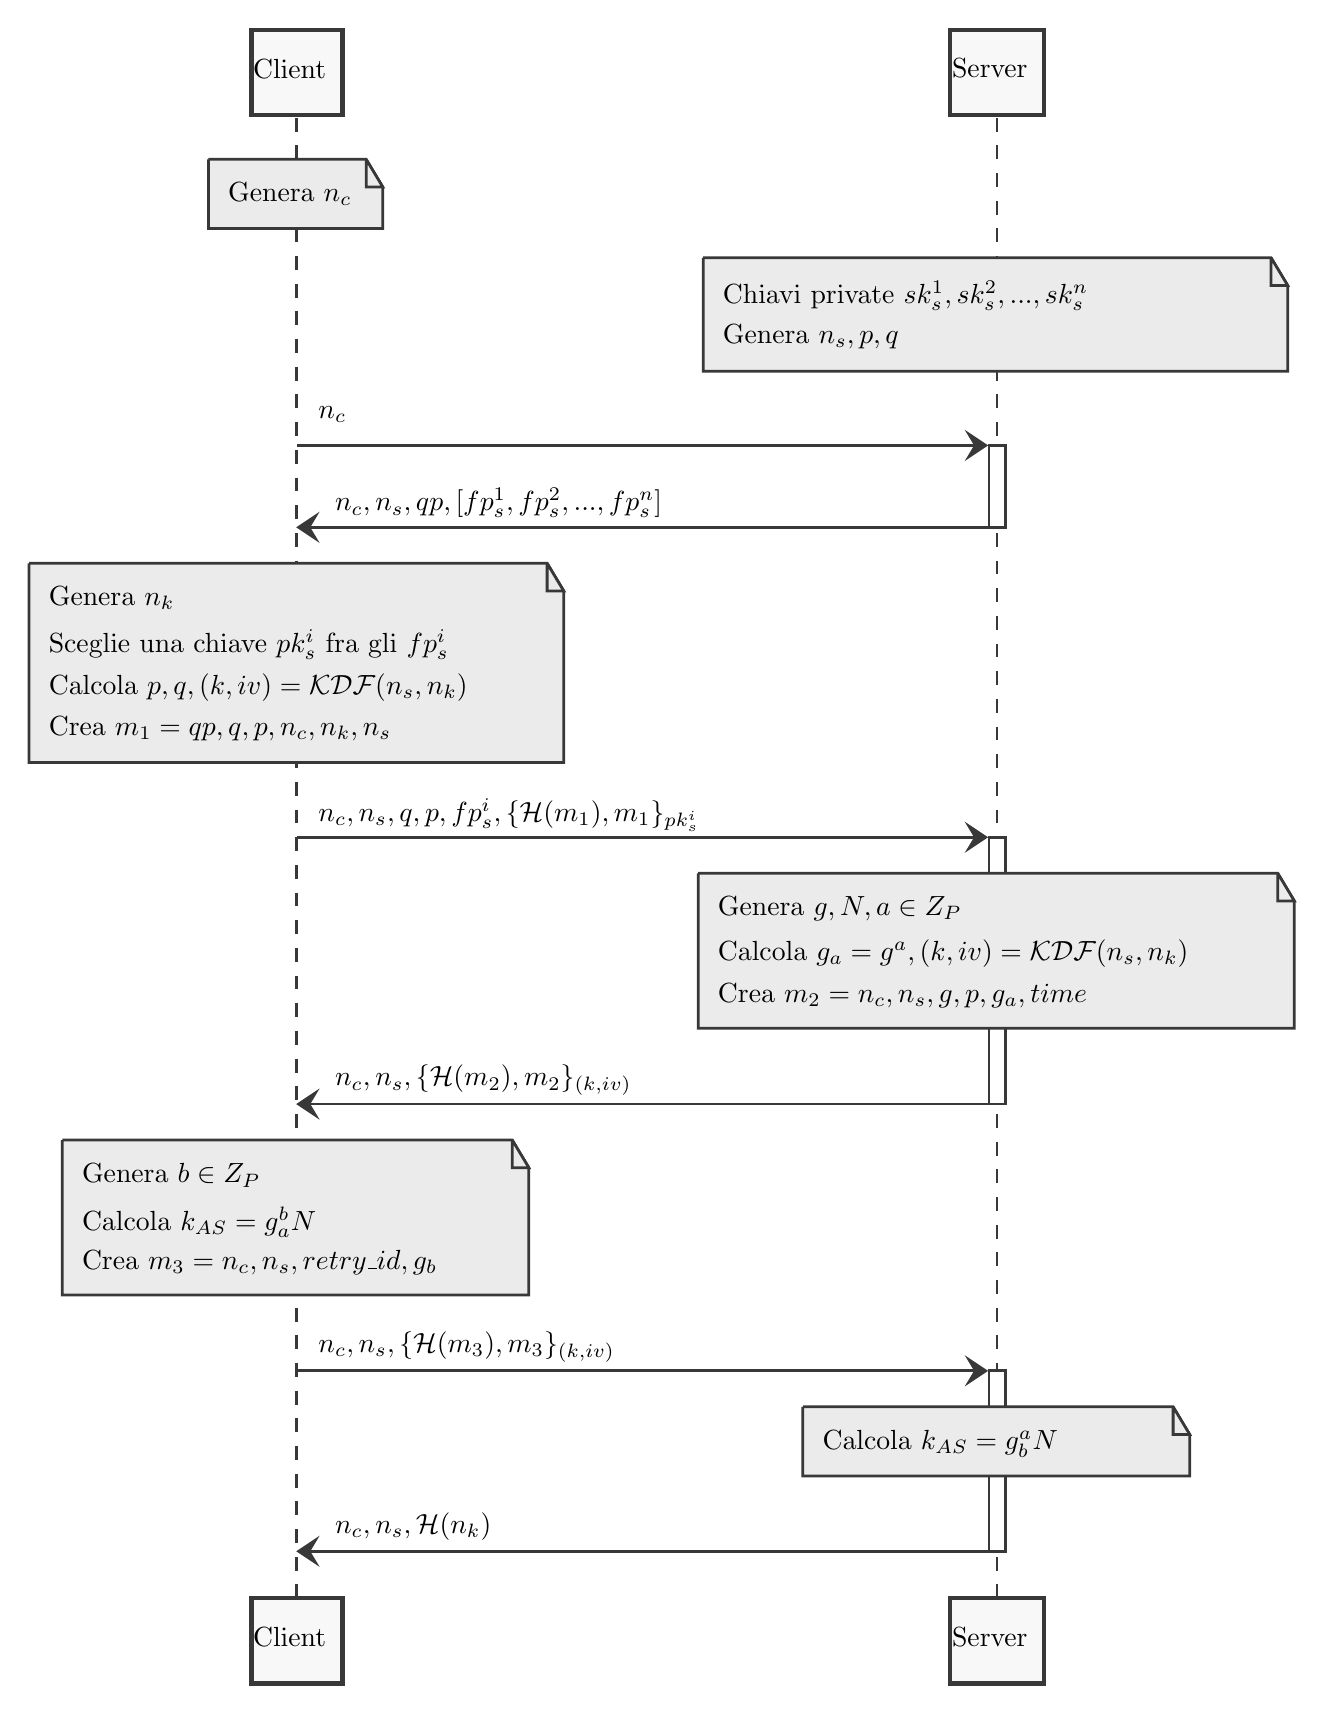
\begin{tikzpicture}[xscale=0.6,yscale=-1
            ,pstyle0/.style={color=plantucolor0001,fill=white,line width=1.0pt}
            ,pstyle1/.style={color=plantucolor0001,line width=1.0pt,dash pattern=on 5.0pt off 5.0pt}
            ,pstyle2/.style={color=plantucolor0001,fill=plantucolor0002,line width=1.5pt}
            ,pstyle3/.style={color=plantucolor0001,fill=plantucolor0004,line width=1.0pt}
            ,pstyle4/.style={color=plantucolor0001,fill=plantucolor0001,line width=1.0pt}
            ,pstyle5/.style={color=plantucolor0001,line width=1.0pt}
        ]
        \draw[pstyle0] (583.0914pt,155.2pt) rectangle (593.0914pt,184.8pt);
        \draw[pstyle0] (583.0914pt,296.8001pt) rectangle (593.0914pt,393.2001pt);
        \draw[pstyle0] (583.0914pt,489.6002pt) rectangle (593.0914pt,554.8002pt);
        \draw[pstyle1] (166pt,36.7999pt) -- (166pt,572.8002pt);
        \draw[pstyle1] (587.8644pt,36.7999pt) -- (587.8644pt,572.8002pt);
        \draw[pstyle2] (139pt,5pt) rectangle (193.8pt,35.7999pt);
        \node at (134pt,12pt)[below right,color=black]{Client};
        \draw[pstyle2] (139pt,571.8002pt) rectangle (193.8pt,602.6001pt);
        \node at (134pt,578.8002pt)[below right,color=black]{Client};
        \draw[pstyle2] (559.8644pt,5pt) rectangle (616.3185pt,35.7999pt);
        \node at (555pt,12pt)[below right,color=black]{Server};
        \draw[pstyle2] (559.8644pt,571.8002pt) rectangle (616.3185pt,602.6001pt);
        \node at (555pt,578.8002pt)[below right,color=black]{Server};
        \draw[pstyle0] (583.0914pt,155.2pt) rectangle (593.0914pt,184.8pt);
        \draw[pstyle0] (583.0914pt,296.8001pt) rectangle (593.0914pt,393.2001pt);
        \draw[pstyle0] (583.0914pt,489.6002pt) rectangle (593.0914pt,554.8002pt);
        \draw[pstyle3] (113pt,51.7999pt) -- (113pt,76.7999pt) -- (218pt,76.7999pt) -- (218pt,61.7999pt) -- (208pt,51.7999pt) -- (113pt,51.7999pt);
        \draw[pstyle3] (208pt,51.7999pt) -- (208pt,61.7999pt) -- (218pt,61.7999pt) -- (208pt,51.7999pt);
        \node at (119pt,56.7999pt)[below right,color=black]{Genera $n_c$};
        \draw[pstyle3] (411pt,87.3999pt) -- (411pt,128.3999pt) -- (763pt,128.3999pt) -- (763pt,97.3999pt) -- (753pt,87.3999pt) -- (411pt,87.3999pt);
        \draw[pstyle3] (753pt,87.3999pt) -- (753pt,97.3999pt) -- (763pt,97.3999pt) -- (753pt,87.3999pt);
        \node at (417pt,92.3999pt)[below right,color=black]{Chiavi private $sk^1_s, sk^2_s, ..., sk^n_s$};
        \node at (417pt,108pt)[below right,color=black]{Genera $n_s, p, q$};
        \draw[pstyle4] (571.0914pt,151.2pt) -- (581.0914pt,155.2pt) -- (571.0914pt,159.2pt) -- (575.0914pt,155.2pt) -- cycle;
        \draw[pstyle5] (166.4pt,155.2pt) -- (577.0914pt,155.2pt);
        \node at (173.4pt,137.6pt)[below right,color=black]{$n_c$};
        \draw[pstyle4] (177.4pt,180.8pt) -- (167.4pt,184.8pt) -- (177.4pt,188.8pt) -- (173.4pt,184.8pt) -- cycle;
        \draw[pstyle5] (171.4pt,184.8pt) -- (587.0914pt,184.8pt);
        \node at (183.4pt,167.2pt)[below right,color=black]{$n_c, n_s, qp, [fp^1_s, fp^2_s, ..., fp^n_s]$};
        \draw[pstyle3] (5pt,197.8pt) -- (5pt,269.8pt) -- (327pt,269.8pt) -- (327pt,207.8pt) -- (317pt,197.8pt) -- (5pt,197.8pt);
        \draw[pstyle3] (317pt,197.8pt) -- (317pt,207.8pt) -- (327pt,207.8pt) -- (317pt,197.8pt);
        \node at (11pt,202.8pt)[below right,color=black]{Genera $n_k$};
        \node at (11pt,218.4pt)[below right,color=black]{Sceglie una chiave $pk^i_s$ fra gli $fp^i_s$};
        \node at (11pt,234pt)[below right,color=black]{Calcola $p, q, (k, iv) = \mathcal{KDF}(n_s, n_k)$};
        \node at (11pt,249.6pt)[below right,color=black]{Crea $m_1 = qp, q, p, n_c, n_k, n_s$};
        \draw[pstyle4] (571.0914pt,292.8001pt) -- (581.0914pt,296.8001pt) -- (571.0914pt,300.8001pt) -- (575.0914pt,296.8001pt) -- cycle;
        \draw[pstyle5] (166.4pt,296.8001pt) -- (577.0914pt,296.8001pt);
        \node at (173.4pt,279.2001pt)[below right,color=black]{$n_c, n_s, q, p, fp^i_s, \{\mathcal{H}(m_1), m_1\}_{pk^i_s}$};
        \draw[pstyle3] (408pt,309.8001pt) -- (408pt,365.8001pt) -- (767pt,365.8001pt) -- (767pt,319.8001pt) -- (757pt,309.8001pt) -- (408pt,309.8001pt);
        \draw[pstyle3] (757pt,309.8001pt) -- (757pt,319.8001pt) -- (767pt,319.8001pt) -- (757pt,309.8001pt);
        \node at (414pt,314.8001pt)[below right,color=black]{Genera $g, N, a \in \mathbb{Z}_P$};
        \node at (414pt,330.4001pt)[below right,color=black]{Calcola $g_a = g^a, (k, iv) = \mathcal{KDF}(n_s, n_k)$};
        \node at (414pt,346.0001pt)[below right,color=black]{Crea $m_2 = n_c, n_s, g, p, g_a, \text{time}$};
        \draw[pstyle4] (177.4pt,389.2001pt) -- (167.4pt,393.2001pt) -- (177.4pt,397.2001pt) -- (173.4pt,393.2001pt) -- cycle;
        \draw[pstyle5] (171.4pt,393.2001pt) -- (587.0914pt,393.2001pt);
        \node at (183.4pt,375.6001pt)[below right,color=black]{$n_c, n_s, \{\mathcal{H}(m_2), m_2\}_{(k, iv)}$};
        \draw[pstyle3] (25pt,406.2001pt) -- (25pt,462.2001pt) -- (306pt,462.2001pt) -- (306pt,416.2001pt) -- (296pt,406.2001pt) -- (25pt,406.2001pt);
        \draw[pstyle3] (296pt,406.2001pt) -- (296pt,416.2001pt) -- (306pt,416.2001pt) -- (296pt,406.2001pt);
        \node at (31pt,411.2001pt)[below right,color=black]{Genera $b \in \mathbb{Z}_P$};
        \node at (31pt,426.8001pt)[below right,color=black]{Calcola $k_{AS} = g^b_a \mod N$};
        \node at (31pt,442.4001pt)[below right,color=black]{Crea $m_3 = n_c, n_s, \text{retry\_id}, g_b$};
        \draw[pstyle4] (571.0914pt,485.6002pt) -- (581.0914pt,489.6002pt) -- (571.0914pt,493.6002pt) -- (575.0914pt,489.6002pt) -- cycle;
        \draw[pstyle5] (166.4pt,489.6002pt) -- (577.0914pt,489.6002pt);
        \node at (173.4pt,472.0002pt)[below right,color=black]{$n_c, n_s, \{\mathcal{H}(m_3), m_3\}_{(k, iv)}$};
        \draw[pstyle3] (471pt,502.6002pt) -- (471pt,527.6002pt) -- (704pt,527.6002pt) -- (704pt,512.6002pt) -- (694pt,502.6002pt) -- (471pt,502.6002pt);
        \draw[pstyle3] (694pt,502.6002pt) -- (694pt,512.6002pt) -- (704pt,512.6002pt) -- (694pt,502.6002pt);
        \node at (477pt,507.6002pt)[below right,color=black]{Calcola $k_{AS} = g^a_b \mod N$};
        \draw[pstyle4] (177.4pt,550.8002pt) -- (167.4pt,554.8002pt) -- (177.4pt,558.8002pt) -- (173.4pt,554.8002pt) -- cycle;
        \draw[pstyle5] (171.4pt,554.8002pt) -- (587.0914pt,554.8002pt);
        \node at (183.4pt,537.2002pt)[below right,color=black]{$n_c, n_s, \mathcal{H}(n_k)$};
    \end{tikzpicture}
    \caption{Diagramma di sequenza dell creazione della chiave di autorizzazione in \gls{mtproto}.
        La funzione hash $\mathcal{H}$ è SHA1.
        $\mathcal{KDF}$ utilizza gli hash di $n_s, n_k$ per generare la chiave temporanea $k$ e il vettore di inizializzazione $iv$}. \label{fig:mtproto-sequence-auth}
\end{figure}


\subsubsection{Dettagli aggiuntivi}
Le due nonce $n_c, n_s$, generate all'inizio dello scambio di messaggi, sono integrate in tutte le comunicazioni successive,
al fine di identificare la sessione.
Si noti che il loro valore è di dominio pubblico. \\

La challenge posta con l'invio di $qp$ e la relativa fattorizzazione ha lo scopo di evitare attacchi DDos.
Un avversario che voglia minare la disponibilità del sistema dovrebbe essere in grado di svolgere un lavoro computazionale
proporzionale al numero di sessioni che si sta creando. \\
Si può parlare di questa strategia come una proof of work semplificata. \\

Il valore di retry\_id parte da 0 e diventa l'hash della chiave di autizzazione precedente qual ora il server
richieda di rinegoziare le chiavi nella stessa sessione.
Questo può accadere, ad esempio, se l'hash della nuova chiave è già presente nella lista di hash di chiavi registrate del server. \\

Il protocollo assume che sia il client che il server verifichino la correttezza dei parametri utilizzati nelle primitive crittografiche.
Eventuali valori che non rientrano negli intervalli definiti sono scartati immediatamente, facendo fallire il protocollo.

